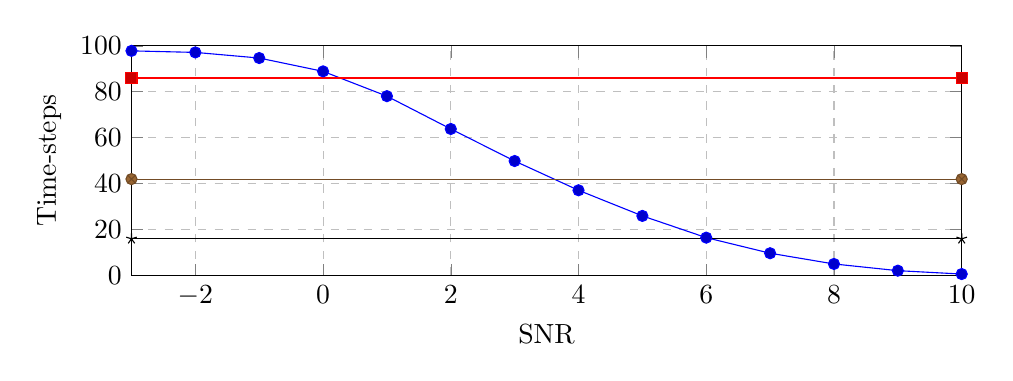
\begin{tikzpicture}

\begin{axis}[
scale=1,
xmin=-3,
xmax=10,
ymin=0,
ymax=100,
ymajorgrids=true,
xmajorgrids=true,
grid style=dashed,
width=\linewidth, height=4.5cm,
xlabel={SNR},
ylabel={Time-steps},
%ylabel shift=-7,
legend cell align={left},
legend pos=north east,
legend style={
	column sep=0mm,
	font=\fontsize{9pt}{9}\selectfont,
},
legend to name=legend-PLatcomp,
legend columns=4,
]

%\addplot
%table {
%-3 96.74
%-2 95.27
%-1 91.81
%0 85.23
%1 75.11
%2 62.16
%3 48.16
%4 34.86
%5 23.24
%6 14.11
%7 7.77
%8 3.57
%9 1.37
%10 0.42
%};
%\addlegendentry{GA}

\addplot
table {
-3 97.80
-2 97.13
-1 94.68
0 88.88
1 78.09
2 63.81
3 49.87
4 37.13
5 25.98
6 16.52
7 9.74
8 5.07
9 2.15
10 0.68
};
\addlegendentry{Proposed}

\addplot
table {
-3 86
10 86
};
\addlegendentry{SC \cite{alamdar2011simplified}}

\addplot
table {
-3 42
10 42
};
\addlegendentry{SC \cite{sarkis2014fast}}

\addplot
table {
-3 16
10 16
};
\addlegendentry{SC \cite{hanif2017fast}}

\end{axis}
\end{tikzpicture}